% @Author: luis
% @Date:   2016-03-30 22:54:01
% @Last Modified by:   luis
% @Last Modified time: 2016-05-01 13:31:42

\documentclass[12pt]{article}
\usepackage{latexsym}
\usepackage{fancyhdr}
\usepackage{amssymb,amsmath,amsthm}
\usepackage[pdftex]{graphicx}
\usepackage{pdfpages}
\usepackage{hyperref}
\usepackage[margin=1in]{geometry}


% Create answer counter to keep track of seperate responses
\newcounter{AnswerCounter}
\newcounter{SubAnswerCounter}
\newcounter{SubSubAnswerCounter}
\setcounter{AnswerCounter}{1}
\setcounter{SubAnswerCounter}{1}
\setcounter{SubSubAnswerCounter}{1}

% Create answer environment which uses counter
\newenvironment{answer}[0]{
  \setcounter{SubAnswerCounter}{1}
  \bigskip
  \textbf{Solution \arabic{AnswerCounter}}
  \\
  \begin{small}
}{
  \end{small}
  \stepcounter{AnswerCounter}
}

\newenvironment{subanswer}[0]{
  \setcounter{SubSubAnswerCounter}{1}
  (\alph{SubAnswerCounter})
}{
 \bigskip
  \stepcounter{SubAnswerCounter}
}

\newenvironment{subsubanswer}[0]{
  \hspace{0.25in}[\roman{SubSubAnswerCounter}]
}{
 \bigskip
  \stepcounter{SubSubAnswerCounter}
}

% Allows easy use of vectors
\newcommand{\vect}[1]{\boldsymbol{#1}}
\newcommand{\deln}[3]{\frac{\partial^{#3} #1}{\partial #2^{#3}}}
\newcommand{\del}[2]{\frac{\partial#1}{\partial #2}}
\newcommand{\bra}[1]{\langle {#1} |}
\newcommand{\ket}[1]{| {#1} \rangle}
\newcommand{\dt}[2]{\langle {#1} | {#2} \rangle}
\newcommand{\braket}[3]{\langle {#1} | {#2} | {#3} \rangle}
\newcommand{\op}[1]{{#1}_{op}}
\newcommand{\opb}[1]{{\bf {#1}}_{op}}


% Custom Header information on each page
\pagestyle{fancy}
\lhead{HUID: 70871564}
\rhead{Luis Perez - \thepage}
\renewcommand{\headrulewidth}{0.1pt}
\renewcommand{\footrulewidth}{0.1pt}

\newcommand{\horrule}[1]{\rule{\linewidth}{#1}}   % Horizontal rule
\title{
    % \vspace{-1in}
    \usefont{OT1}{bch}{b}{n}
    \normalfont \normalsize \textsc{Harvard University} \\ [25pt]
    \horrule{0.5pt} \\[0.4cm]
    \huge Physics 143a: Quantum Mechanics I \\ [20pt]
    \normalfont \normalsize Problem Set 9
    \horrule{2pt} \\[0.5cm]
}
\author{
    \normalfont                 \normalsize
        Luis Antonio Perez\\[-3pt]    \normalsize
}
\date{\today}

\begin{document}
\maketitle
\pagebreak
\begin{answer}
We consider a perturbed system known as the anharmonic oscillator. Recall that for the harmonic oscillator we have the Hamiltonian
$$
H_0 = \frac{p^2}{2m} + \frac{1}{2} m\omega^2x^2
$$
which has energy eigenstates $E_n = (\frac{1}{2} + n)\hbar \omega$ and eigenfunctions $\ket{n}$.

\begin{subanswer}
We now perturb the state by adding the Hamiltonian $H' = cx^4$. This new system is known as the anharmonic oscillator. We wish to solve the TISE:
$$
H\ket{\psi_n} = E_n \ket{\psi_n}
$$
According to first order perturbation theory, we can approximate $E_n$ with the following:
$$
E_n = E_n^0 + E_n^1
$$
where $E_n^0 = (\frac{1}{2} + n)\hbar \omega $ and:
$$
E_n^1 = \braket{n}{H'}{n}
$$
In order to compute the above, we first calculate $ax^4$ using raising and lowering operators, recalling that $x = \sqrt{\frac{\hbar}{2m\omega}}(a^\dag + a)$.
\begin{align*}
cx^4 &= c\left(\frac{\hbar^2}{4m^2\omega^2} \right)(a^\dag + a)^4 \\
&=c\left(\frac{\hbar^2}{4m^2\omega^2} \right)[(a^\dag)^4 + a^4 + (a^\dag)^3a + a^3a^\dag + (a^\dag)^2aa^\dag + a^2a^\dag a + a^\dag a (a^\dag)^2 + a a^\dag a^2 + a(a^\dag)^3 + a^\dag a^3 \\
&+ (a^\dag)^2a^2 + a^2(a^\dag)^2 + (a^\dag a)^2 + (a a^\dag)^2 + a(a^\dag)^2a + a^\dag a^2 a^\dag] \\
&= c\left(\frac{\hbar^2}{4m^2\omega^2} \right)[(a^\dag)^4 + a^4 + (a^\dag)^2N + a^2N^\dag + a^\dag N a^\dag + a^2 N + N (a^\dag)^2 + a N a + N^\dag (a^\dag)^2 + N a^2 \\
&+ a^\dag N a  + a N^\dag a^\dag + N^2 + (N^\dag)^2 + N^\dag N + N N^\dag]
\end{align*}
where $N = a^\dag a$. Let us recall the following facts:
\begin{align*}
a^\dag \ket{n} &=  \sqrt{n+1}\ket{n+1} \\
a\ket{n} &= \sqrt{n}\ket{n-1} \\
N\ket{n} &= n\ket{n} \\
N^\dag \ket{n} &= (n+1)\ket{n}
\end{align*}
with the above, we can apply the operator. We use the fact that
$\dt{m}{n} = \delta_{mn}$ to note that any operator above in the expansion which does not maintain the same eigenstate will be null. We drop these terms:
\begin{align*}
\braket{n}{x^4}{n} &= \frac{\hbar^2}{4m^2\omega^2} \braket{n}{a^\dag N a + a N^\dag a^\dag + N^2 + (N^\dag)^2 + N^\dag N + N N^\dag}{n} \\
&= \frac{\hbar^2}{4m^2\omega^2} \left[n(n-1) + (n+2)(n+1) + n^2 + (n+1)^2  + 2n(n+1) \right] \\
&= \frac{3\hbar^2}{4m^2\omega^2} \left[2n^2 + 2n + 3 \right]
\end{align*}
Therefore, putting all of the above together, we arrive at the following conclusion:
$$
E_n \approx (\frac{1}{2} + n)\hbar \omega + c\frac{3\hbar^2}{4m^2\omega^2}[2n^2 + 2n + 1]
$$
\end{subanswer}

\begin{subanswer}
First note that we rebaled our constant from $a$ to $c$, so let us not confuse the question.

If the non-degenerate perturbation theory above is to be valid, we require that:
\begin{align*}
|E_m^0 - E_n^0| >> \braket{m}{H'}{n} \\
\implies |m - n|\hbar \omega >> c \braket{m}{x^4}{n}
\end{align*}
Note that $m,n$ are both integers, so if $m \neq n$, the smallest possible LFS is $\hbar \omega$. However, note that the RHS is $0$ whenever $|m - n| > 4$ (as all dot products are among states with distinct quantum numbers). Therefore we only consider states where
$ 1 \leq |m - n| \leq 4$, and we have the following relation:
$$
\braket{m}{x^4}{n} = \frac{\hbar^2}{4m^2\omega^2} O(n^2)
$$
so we require, at least, that:
$$
c << \frac{4m^2\omega^3}{h\bar O(n^2)}
$$
so $c$ must be small, extremely small, and for higher energy levels, the smaller it must be in order for our approximation to be correct.
\end{subanswer}

\begin{subanswer}
We first calculate the difference between adjacent energy levels $E_n$ and $E_{n+1}$, which results in the following:
$$
E_{n+1} - E_n = \hbar \omega + c\frac{3\hbar^2}{2m^2 \omega^2}(n+1)
$$
This is the excitation energy for our anharmonic oscillator. Furthermore, we note that the excitation energy for the original harmonic oscillator is $\hbar \omega$, and the excitation energy from $0 \to 1$ of our new system is:
$$
E_1 - E_0 = \hbar\omega + c \frac{3\hbar^2}{2m^2 \omega^2}
$$

We assume that the overall oscillator frequency is given by $\omega'$ where the energy is $\Delta E = \hbar \omega'$, so solving for $\omega'$, we have:
$$
\omega' = \omega + c\frac{3\hbar }{2m^2\omega^2}
$$
where $\omega$ is the frequency of the harmonic oscillator system we perturbed to obtain the anharnomic oscillator.
\end{subanswer}
\end{answer}

\begin{answer}
We now consider the relativistic kinetic energy correction to the hydrogen fine structure. The perturbation Hamiltonian is:
$$
H' = -\frac{p^4}{8m^3c^2}
$$

\begin{subanswer}
We check whether the above Hamiltonian commute with $L^2,L_z,S^2,S_z,J^2,J_z$. Note that it is immediate that it must commute with $S^2, S_z$ since neither of these has a position representation and each acts on an abstract spin, separate from the position representation of the wave-function. We note that $H'$ acts only on the position coordinates. Therefore, we can conclude that:
\begin{align*}
[H',S^2] &= 0\\
[H',S_z] &= 0
\end{align*}
We're now proceed to $L^2$ and $L_z$. Note that $H'$ is spherically symmetrical, so it is also immediate that it must commute with $L^2, L_z$. Therefore:
\begin{align*}
[H', L^2] = 0 \\
[H', L_z] = 0
\end{align*}
Finally, we take $J = L + S$ and consider $J^2 = (L + S)^2$ and $J_z = L_z + S_z$. Note the following:
\begin{align*}
[H', J_z] &= [H', L_z] + [H',S_z] = 0 \\
[H', J^2] &= [H', J^2] + [H', L^2] + 2[H', L\cdot S] = 0 + 2([H', L_xS_x] + [H', L_yS_y] + [H', L_z,S_z])
\end{align*}
Note that $[H', L_iS_i] = [H',L_i]S_i + L_i[H',S_i] = 0$, therefore,
$$
[H', J^2] = 0
$$
we conclude that all of the above commute.
\end{subanswer}

\begin{subanswer}
The consequence is that we don't need to use degenerate perturbation theory, despite the fact that we have degenerate energy states. Instead, thanks to the theorem discussed in lecture and in the textbook (see Section 6.2.1), we have operators which commute with the perturbation Hamiltonian and for which the eigenstates of the original Hamiltonian are also eigenstates with distinct eigenvalues. This means that we can directly calculate the needed matrix elements by using ordinary (non-degenerate) perturbation theory on the good eigenstates that are both eigenstates of $H_0$ and $A$ (we describe $A$ later) to calculate the first-order perturbation to the energy. In the case where we pick $A$ to be a combination of $(L_z,L^2,S^2,S_z)$ (so, for example, $A = L^2L_zS^2S_z$), we use the uncoupled basis $\ket{n; l, m_l; s, m_s}$ to calculate the matrix elements $\langle H' \rangle$. Note that we have, for $A$ of the form described:
$$
A\ket{n; l, m_l; s, m_s} = \hbar^6 l(l+1)s(s+1)m_lm_s\ket{n; l, m_l; s, m_s}
$$
which, for a fixed $n$, all have distinct eigenvalues since each is of the $2n^2$ states for $n$ is uniquely specified by a set $l,s,m_l,m_s$ and produces a unique value $ls(l+1)(s+1)m_lm_s$.


Additionally, we can also take $A$ to be a combination of $J^2, J_z$ (such as $A = J^2J_z$), and we use the coupled basis $\ket{n; (l,s) j, m_j}$. Note that for the $A$ of this form we have:
$$
A \ket{n; (l,s) j, m_j} =  j(j+1)m_j\ket{n; (l,s) j, m_j}
$$
so that for fixed $n$, ass distinct eigenvalues.

In either scenario, both basis are ``good'' states and we can use non-degenerate first-order perturbation theory.
\end{subanswer}

\begin{subanswer}
We follow the presentation in Griffith and select the uncoupled basis with the commutator $L^2$ or $L_z$. By part (b), we can use non-degenerate first-order perturbed theory. We also recall that $p^2$ is Hermitian and begin with a general basis $\psi$. Furthermore, we recall that by TISE, $p^2 \ket{\psi} = 2m(E - V)\psi$.
\begin{align*}
E_{nlm_lsm_s}^1 &= \langle H' \rangle \\
&= -\frac{1}{8m^3c^2}\braket{\psi}{p^2 p^2}{\psi} \\
&= -\frac{1}{8m^3c^2}\dt{p^2 \psi}{p^2 \psi} \\
&= -\frac{1}{2mc^2}\langle(E-V)^2 \rangle \\
&= -\frac{1}{2mc^2}(E^2 - 2E\langle V \rangle + \langle V^2 \rangle)
\end{align*}
We now recall that for hydrogen we have:
$$
V(r) = - \frac{e^2}{4\pi\epsilon_0 r}
$$
which leads to:
$$
E_{nlm_l}^1 = -\frac{1}{2mc^2}\left[E_n^2 + 2E_n\left(\frac{e^2}{4\pi\epsilon_0}\right)\left\langle \frac{1}{r} \right\rangle + \left(\frac{e^2}{4\pi\epsilon_0}\right)^2\left\langle \frac{1}{r^2} \right\rangle \right]
$$
where $E_n$ is the energy of the state $\ket{n;l,m_l;s,m_s}$ under the standard Hamiltonian for the hydrogen atom. We note that, according to Griffith, we have:
$$
\left\langle \frac{1}{r} \right \rangle = \frac{1}{n^2 a_B}
$$
and
$$
\left \langle \frac{1}{r^2} \right \rangle = \frac{1}{(l + 1/2)n^3a^2}
$$
so we conclude that the perturbed energy contributions are:
$$
E_{nlm_l}^1 = -\frac{1}{2mc^2}\left[E_n^2 + 2E_n\left(\frac{e^2}{4\pi\epsilon_0}\right)\left(\frac{1}{n^2 a_B} \right) + \left(\frac{e^2}{4\pi\epsilon_0}\right)^2\left(\frac{1}{(l + 1/2)n^3a^2}\right)\right]
$$
and substituting $a_B$ and simplifying:
$$
E_{nlm_l}^1 = -\frac{E_n^2}{2mc^2}\left[ \frac{4n}{l+1/2} - 3\right]
$$
which gives us the lowest order shift for each energy level. We note explicitly that it depends only on $n,l$ and we relabel the correction as:
$$
E_{rel}^1 = \frac{(E_n)^2}{2mc^2}\left[3 - \frac{4n}{l+1/2}\right]
$$
in preparation for future problems.
\end{subanswer}
\end{answer}

\begin{answer}
We now consider the spin-orbit interaction, which has perturbation Hamiltonian:
$$
H' = \frac{1}{2m^2c^2}\frac{1}{r}\del{V}{r} L \cdot S
$$

\begin{subanswer}
Note that we now check whether $H'$ commutes with $L_z, S_z$ (it does not!)
\begin{align*}
[L\cdot S, L_z] &= [L_xS_x, L_z] + [L_yS_y, L_z] + [L_zS_z, L_z] \\
&= \underbrace{L_x[S_x,L_z]}_{=0} + [L_x,L_z]S_x + \underbrace{L_y[S_y,L_z]}_{=0} + [L_y,L_z]S_y + \underbrace{L_z[S_z, L_z]}_{=0} + \underbrace{[L_z,L_z]S_z}_{= 0} \\
&= -i\hbar L_yS_x + i\hbar L_xS_y
\end{align*}
and by a similar argument, where we simply substitute $L_z$ with $S_z$, we have:
$$
[L \cdot S, S_z] = i\hbar[S_xL_y - S_yL_x]
$$
neither of which is null. Therefore $H'$ and $L_z,S_z$ don't commute.

Next, we show that it nonetheless commutes with $L^2, S^2, J^2,$ and $J_z$. The fact that $J_z$ commutes follows from:
$$
[L \cdot S, J_z] = [L \cdot S, L_z] + [L \cdot S, S_z] = i\hbar [L_xS_y - L_yS_x + S_xL_y - S_yL_x]  = 0
$$
recalling that $L$ and $S$ commute. Next, we recall that $[L_i, L^2] = 0$ and that $S_i$ and $L^2$ commute to arrive at the following:
$$
[L \cdot S, L^2] = \sum_{i \in \{x,y,z\}} [L_iS_i, L^2] = \sum_{i \in \{ x,y,z\}} L_i\underbrace{[S_i,L^2]}_{=0} + \underbrace{[L_i,L^2]}_{=0}S_i = 0
$$
and, by a similar argument as above except where we replace $L^2$ with $S^2$ and recall that $[S_i,S^2] = 0$ and $L_i$ and $S^2$ commute, we have
$$
[L \cdot S, S^2] = 0
$$
With the above, we can calculate the following:
$$
[L \cdot S, J^2] = [L \cdot S, L^2] + [L \cdot S, S^2] + 2[L \cdot S, L\cdot S]  = 0
$$
so we have that the perturbation Hamiltonian $H'$ commutes with only $J_z, L^2, S^2, J^2$.
\end{subanswer}

\begin{subanswer}
In this scenario, the conclusions is that we know for a fact that the coupled basis ($\ket{n; (ls) j, m_j}$) are ``good'' states and can be used with non-degenerate first-order perturbation theory to approximate first-order correction terms due to the perturbed Hamiltonian. The reason for this is that those states are eigenvectors of both the original Hamiltonian for the hydrogen atom as well as of the operator $A$ consisting of a combination of $J_z, J^2$. However, the uncoupled basis can't be used since $S_z, L_z$ no longer commute with the perturbation Hamiltonian, so any $A$ containing them wont' commute.

In the case where it does work (for examples, $A = J_zJ^2$), we note that:
$$
A \ket{n; (l,s) j, m_j} =  j(j+1)m_j\ket{n; (l,s) j, m_j}
$$
all with distinct eigenvalues for a given $E_n$. Therefore, the coupled basis is a ``good'' basis and can be used to calculate the first-order correction term caused by the perturbation Hamiltonian.
\end{subanswer}

\begin{subanswer}
We use the coupled basis as described above to calculate the matrix elements. We begin by finding the eigenvalues for $L \cdot S$ by noting that $L\cdot S = J^2 - L^2 - S^2$ so the eigenvalues are $\frac{\hbar^2}{2}[j(j+1) - l(l+1) - \frac{3}{4}]$. We can then calculate the matrix elements:
\begin{align*}
\langle H' \rangle &= \frac{1}{2m^2c^2}\langle \frac{1}{r}\del{V}{r} L \cdot S \rangle \\
&= \frac{\hbar^2[j(j+1) - l(l+1) - 3/4]}{16 \pi \epsilon_0 m^2c^2}\left \langle \frac{1}{r^3} \right \rangle \\
&= \frac{\hbar^2[j(j+1) - l(l+1) - 3/4]}{16 \pi \epsilon_0 m^2c^2} \frac{1}{l(l+1/2)(l+1)n^3a_B^3}\tag{we used textbook results here} \\
&= \frac{(E_n)^2}{mc^2} \left\{\frac{n[j(j+1) - l(l+1) - 3/4]}{l(l+1/2)(l+1)} \right\} = E_{so}^1
\end{align*}
where $E_n$ is the energy of the unperturbed Hamiltonian in state $n$. Note that we can further simplify the above using the fact that $j = l \pm 1/2$ to simplify the numerator:
\begin{align*}
(l \pm 1/2)(l + 1 \pm 1/2) - l(l+1) - 3/4 &= l(l+1) + 1/4 \pm 1/2(l + l + 1) - -l(l+1) 3/4 \\
&= \pm1/2(2l + 1) -1/2 \\
&= l \text{ or } -(l+1)
\end{align*}
And so, by the above, we have:
\begin{align*}
E_{so}^1 = \begin{cases}
\frac{n(E^0_n)^2}{mc^2 (l+1/2)(l+1)} & j = l + 1/2 \\
-\frac{n(E^0_n)^2}{mc^2 l(l+1/2)} & j = l - 1/2
\end{cases}
\end{align*}
Note that the term above is ambiguous for the case when $l = 0$ (as we obtain an indeterminate form $0/0$. We resolve this issue in the next problem by introducing the ``Darwin Term'').
\end{subanswer}
\end{answer}

\begin{answer}
We now consider the ``Darwin Term'', so named because it allows us to handle the case where $l = 0$ and ``survive'' all of this algebra! We're told that the perturbation Hamiltonian is:
$$
H' = \frac{\hbar^2 e^2}{8m^2c^2 \epsilon_0}\delta^3(\vect{r})
$$

\begin{subanswer}
Note that $H'$ is spherically symmetrical and defined only for position coordinates $\vect{r}$, and therefore for similar reasons as for the relativity correction, $H'$ here commutes with all $J_z, J^2, L_z, L^2, S_z, S^2$. We do not repeat the argument for succinctness.
\end{subanswer}

\begin{subanswer}
The exact same argument that applied to the relativity correction applies here, and therefore we have that both the coupled and uncoupled basis are ``good'' basis and we can use either to calculate the first term correction.
\end{subanswer}

\begin{subanswer}
We use the coupled basis, which we write as $\psi_{nlm_l}$ (since spin is not affected by $H'$, so we can ignore it), though as argued above, either basis works well. Then we can take the expected values of $H'$:
\begin{align*}
\langle H' \rangle &= \braket{\psi_{nlm_l}}{H'}{\psi_{nlm_l}} \\
&= \frac{\hbar^2 e^2}{8m^2c^2\epsilon_0}|\Psi_{nlm_l}(\vect{0})|^2
\end{align*}
Then we note that for $l > 0$, $\psi_{nlm_l}(\vect{0}) \propto R_{nl}^2(\vect{0})$ which in the limit of $r \to 0$, we have $\lim_{r \to 0 } R_{nl}(\vect{r}) \propto r^l$ so that the term here actually only comes into play for the values where $l = 0$ (it will vanish if $l \neq 0$). In that scenario, we have $\psi(\vect{0}) = \sqrt{\frac{1}{\pi}}\left(\frac{1}{na_B} \right)^{3/2}$ so we have:
$$
\langle H' \rangle = \frac{\hbar^2 e^2}{8 \pi m^2c^2\epsilon_0^2 n^3 a_B^3} = 2n \frac{(E_n^0)^2}{mc^2} = E_D
$$
which matches the correction from the previous problem for $l = 0$ and $j = 1/2$. The above is the lowest order shift for the energy, according to perturbation theory, in the case where $l = 0$.
\end{subanswer}
\end{answer}

\begin{answer}

\begin{subanswer}
We now consider the sum of the above three correction terms. First, we note that in the case when $l = 0$, the contributions from the spin-orbit interaction are $0$ because as the electron enter the nucleus the potential begins to decrease. This means that the term $\left\langle 1/r^3 \right\rangle$ would be a large, but finite value. Furthermore, the electron would begin to achieve relativistic speeds, therefore the correction due to relativity should be small. Therefore, we conclude that for $l = 0$, the contributions from spin-orbit coupling vanish.

However, note that for $l = 0$, the Darwin contribution is non-zero and precisely makes up for the lack of spin-orbit contribution. In the other cases, the Darwin contribution is exactly $0$ . Therefore, when summing these two contributions we see that the Darwin contributions fills in the gap left by the spin-orbit coupling calculations for $l = 0$.

More explicitly, for $l = 0 \implies s = 1/2$, we keep only the relativistic and Dawrwin terms:
$$
E_{n,0,1/2} = E_{rel} + E_D = \frac{(E_n^0)^2}{mc^2}\left[3/2 - 4n + 2n \right] = \frac{(E_n^0)^2}{2mc^2}[3 - 4n]
$$
and for the case when $l \neq 0$ the Darwin term is null and the contributions come from the spin-orbit coupling, so using the fact that $j = l \pm 1/2$ we have the following
\begin{align*}
E_n^1 &= E_{rel} + E_{so} = \frac{(E_n^0)^2}{mc^2}\left[\frac{3}{2} - \frac{2n}{l+1/2} +  \frac{n[j(j+1) - l(l+1) - 3/4]}{l(l+1/2)(l+1)}\right] \\
&= -\frac{(E_0^0)^2}{mc^2}\frac{1}{n^4} \left[\frac{2n}{l+1/2} - \frac{n[j(j+1) - l(l+1) - 3/4]}{l(l+1/2)(l+1)} - \frac{3}{2}\right] \\
&= -\frac{(E_0^0)^2}{mc^2}\frac{1}{n^4} \left[\frac{n[-j(j+1) + 3l(l+1) + 3/4]}{l(l+1/2)(l+1)} - \frac{3}{2}\right]
\end{align*}
We attempt to simplify the inner term in the above expression to get rid of all $l$s. We first use $l = j - 1/2$, and note that the denominator takes the form $(j-1/2)j(j+1/2)$ and get:
\begin{align*}
3l(l+1) + 3/4 - j(j+1) &= 3(j-1/2)(j+1/2) + 3/4 - j(j+1) \\
&= 3j(j-1/2) +3/2j - 3/4 + 3/4 - j(j+1) \\
&= 3j(j-1/2) - j(-3/2 + j + 1) \\
&= 3j(j-1/2) - j(j-1/2) \\
&= 2j(j-1/2)
\end{align*}
which means we have:
$$
E_n^1 = \frac{(E_0^0)^2}{mc^2}\frac{1}{n^4}\left[\frac{2n}{j+1/2} - \frac{3}{2} \right]
$$
In the case where $l = j + 1/2$, we proceed with similar simplifications, noting that the denominators takes the form $(j+1/2)(j+1)(j + 3/2)$ and we get:
\begin{align*}
3l(l+1) + 3/4 - j(j+1) &= 3(j+1 - 1/2)(j+3/2) + 3/4 - j(j+1) \\
&= 3(j+3/2)(j+1) - 3/2(j + 3/2)+ 3/4 - j(j+1) \\
&= 3(j+3/2)(j+1) - 3/2(j + 1 + 1/2)+ 3/4 - j(j+1) \\
&= 3(j+3/2)(j+1) - 3/2(j + 1) -3/4 + 3/4 - j(j+1) \\
&= 3(j+3/2)(j+1) - (j + 1)(j + 3/2) \\
&= 2(j+3/2)(j+1)
\end{align*}
which means we have:
$$
E_n^1 = \frac{(E_0^0)^2}{mc^2}\frac{1}{n^4}\left[\frac{2n}{j+1/2} - \frac{3}{2} \right]
$$
So in either scenario, we obtain the same solution. We can make explicit the dependence on $n,j$ by labeling:
$$
E_{n,j}^1 = \frac{(E_0^0)^2}{mc^2}\frac{1}{n^4}\left[\frac{2n}{j+1/2} - \frac{3}{2} \right]
$$
we can further simplify the above to make the fine-structure constant explicit (using the Bohr) formula, to obtain:
$$
E_{nj} = -\frac{13.6 eV}{n^2}\left[1 + \frac{\alpha^2}{n^2}\left(\frac{n}{j+1/2} - \frac{3}{4} \right) \right]
$$
\end{subanswer}

\begin{subanswer}
Apologies for the poor quality. Figure \ref{ref:hydrogen_energy_levels}.

\begin{figure}[h!]
\centering
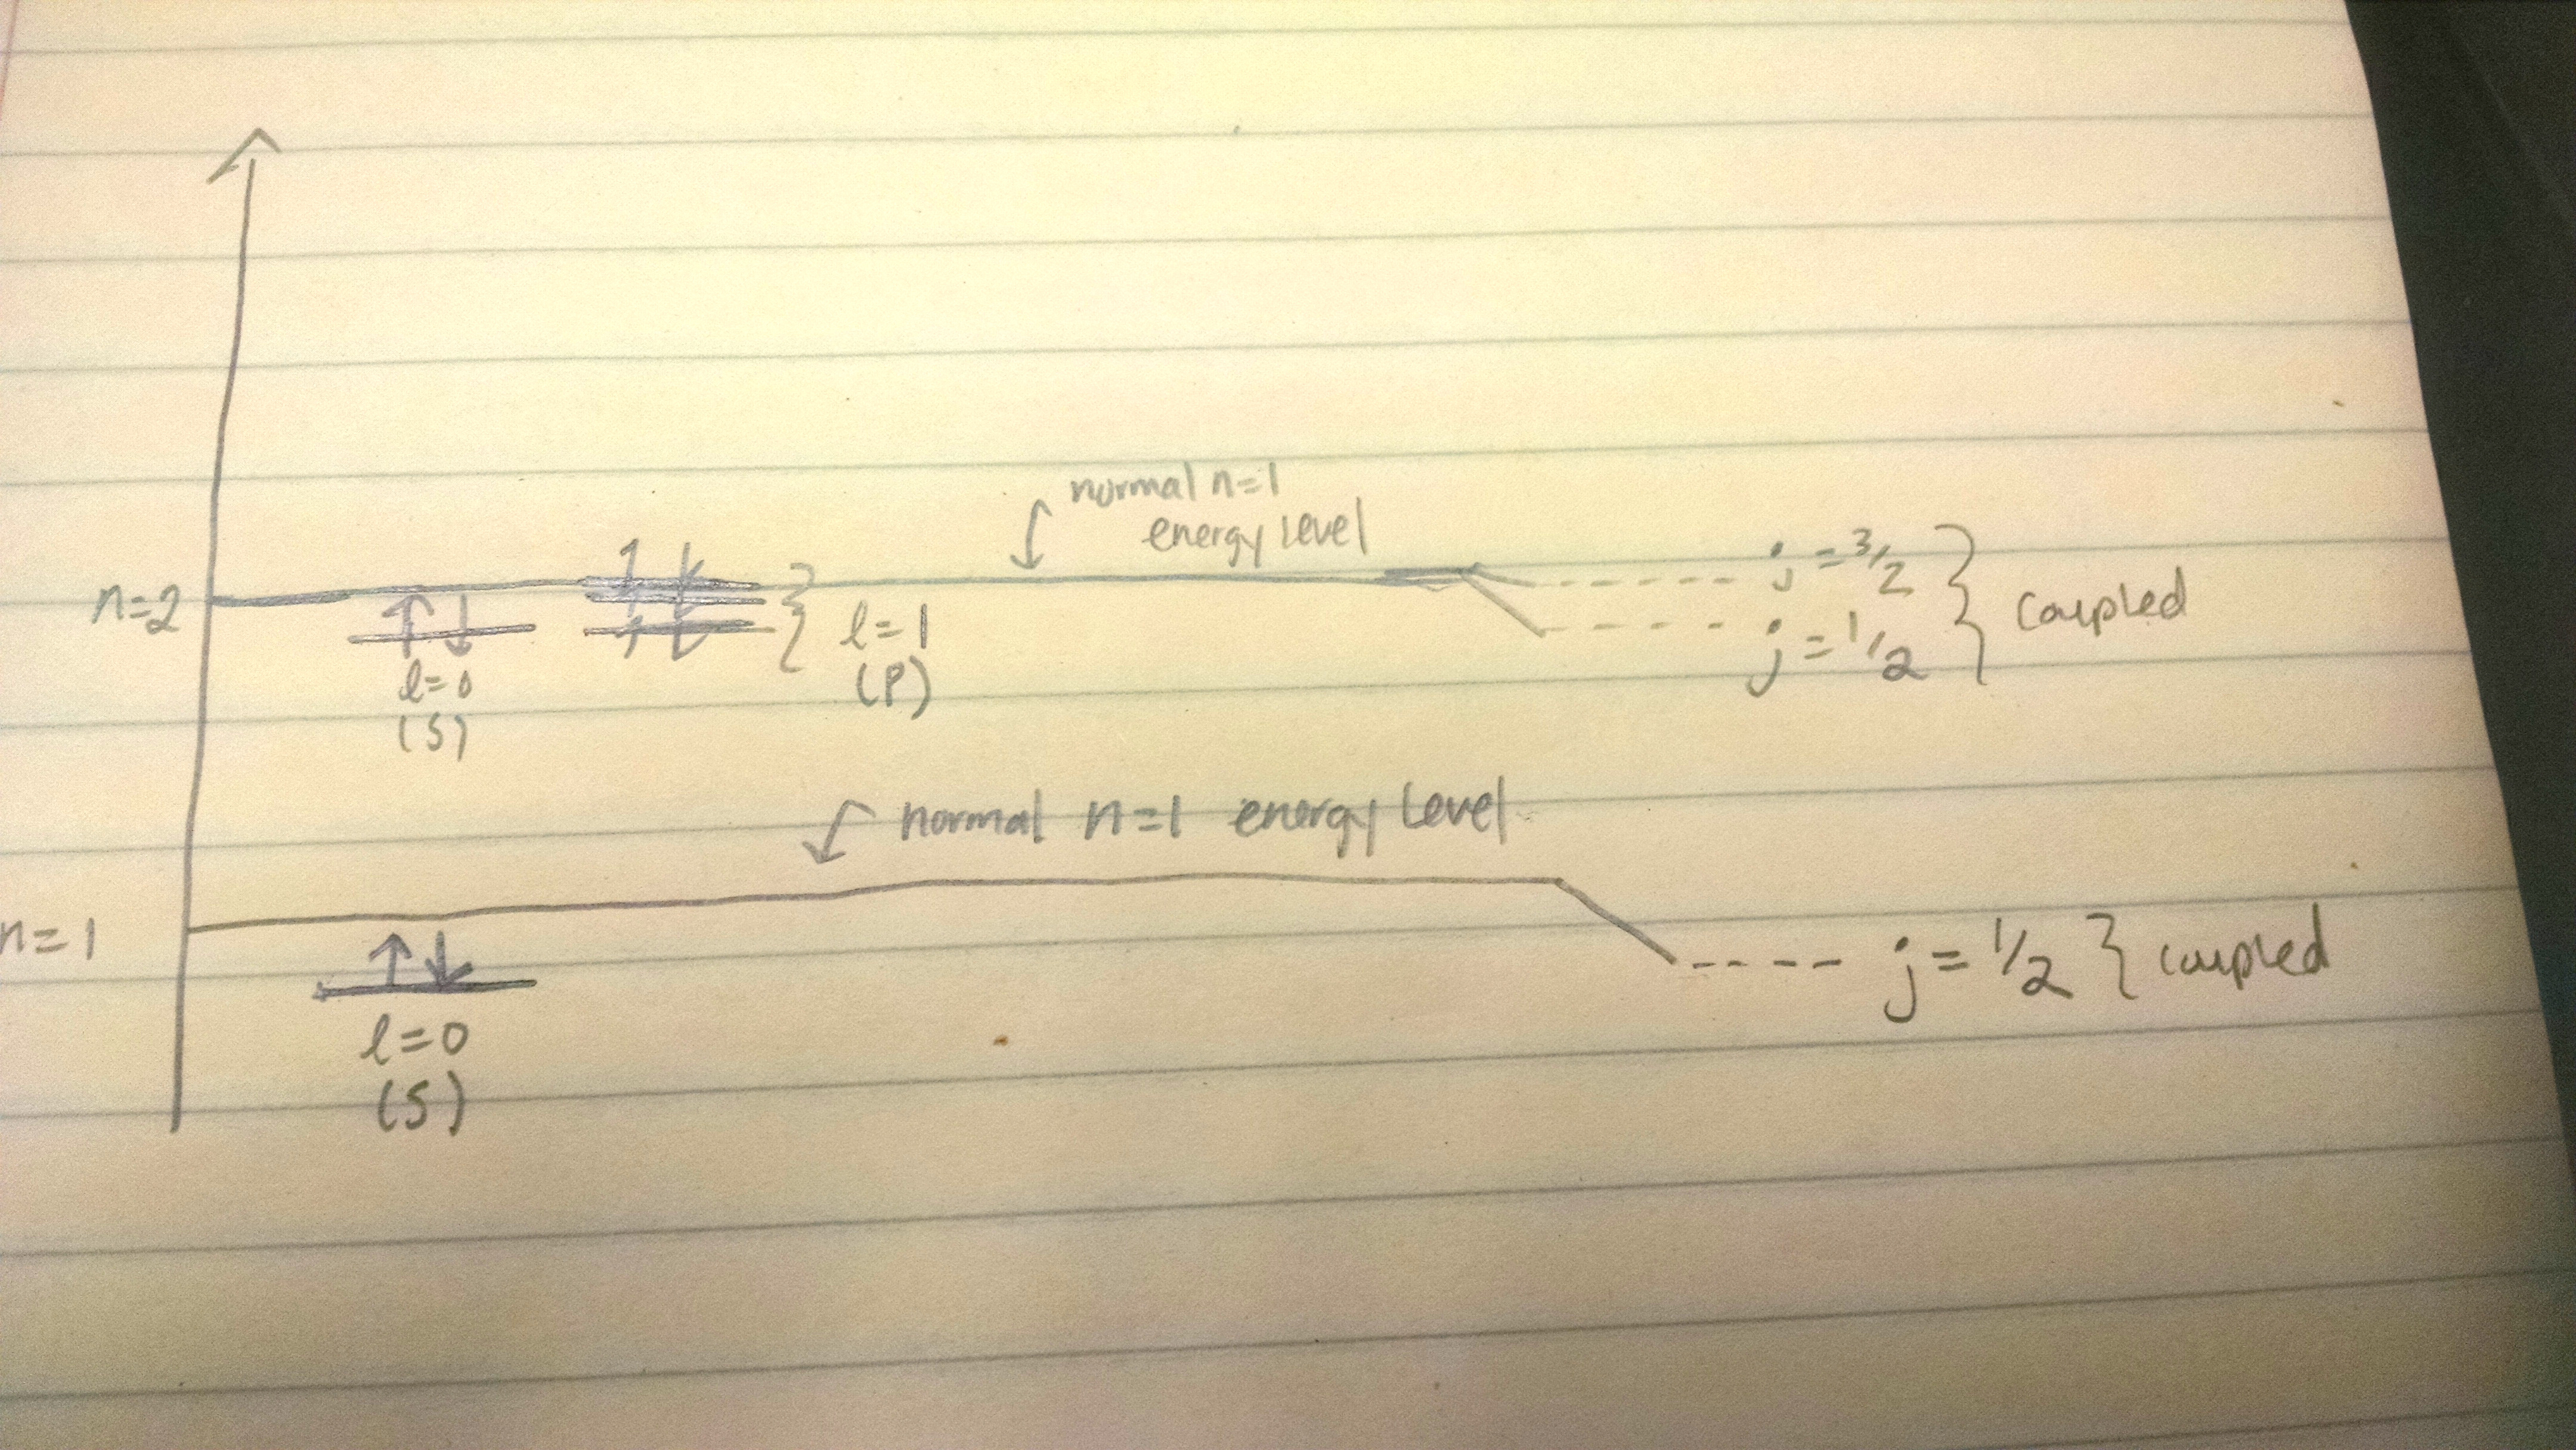
\includegraphics[scale=0.1]{energy_levels.jpg}
\caption{Energy Levels for Hydrogen Atom with Fine-structure effects included}
\label{ref:hydrogen_energy_levels}
\end{figure}
\end{subanswer}
\end{answer}

\begin{answer}
We are now tasked with simplifying the following term so that it matches with the above calculated energy!
$$
E_{nj} = mc^2 \left\{\left[1 + \left(\frac{\alpha}{n - (j + 1/2) + \sqrt{(j+1/2)^2 - \alpha^2}} \right)^2 \right]^{-1/2} - 1 \right\}
$$
We begin by simplifying simpler terms:
\begin{align*}
\sqrt{(j+1/2)^2 - \alpha^2} &= (j+1/2)\sqrt{1 - \frac{\alpha^2}{(j+1/2)^2}} \\
&\approx (j+1/2)\sqrt{1 - \frac{\alpha^2}{(j+1/2)^2} + \frac{\alpha^4}{4(j_1/2)^4}} \tag{add a small term $O(\alpha^4)$} \\
&\approx (j+1/2)\left[1 - \frac{\alpha^2}{2(j+1/2)^2} \right] \\
&= (j+1/2) - \frac{\alpha^2}{2j+1}
\end{align*}
Plugging into its respective location, we have:
\begin{align*}
\left[1 + \left(\frac{\alpha}{n - (j + 1/2) + \sqrt{(j+1/2)^2 - \alpha^2}} \right)^2\right]^{-1/2} &\approx \left[ 1 + \left(\frac{\alpha}{n - \frac{\alpha^2}{2j+1}}\right)^2\right]^{-1/2} \\
&=\left[ 1 + \frac{\alpha^2}{n^2} \left[\frac{1}{1 - \frac{\alpha^2}{2n(j+1/2)}} \right]^2\right]^{-1/2}\\
&\approx \left[ 1 + \frac{\alpha^2}{n^2}\left[1 + \frac{\alpha^2}{2n(j+1/2)} \right]^2\right]^{-1/2} \tag{$1 - x^2 \approx 1 \implies 1+x \approx \frac{1}{1-x}$} \\
&\approx \left[ 1 + \frac{\alpha^2}{n^2}\left[1 + \frac{\alpha^2}{n(j+1/2)} \right]\right]^{-1/2} \tag{dropping higher order terms} \\
&\approx 1 - \frac{1}{2} \frac{\alpha^2}{n^2}\left(1 + \frac{\alpha^2}{n(j + 1/2)}\right) + \frac{3}{8}\frac{\alpha^4}{n^4} \tag{expanding using power series} \\
&=1 - \frac{\alpha^2}{2n^2} + \frac{\alpha^4}{2n^4}\left(\frac{-n}{j+1/2} + \frac{3}{4} \right)
\end{align*}
Pluggin the above result into the full terms, we have:
\begin{align*}
E_{nj} &= -\frac{mc^2\alpha^2}{2n^2}\left\{1 + \frac{\alpha^2}{n^2} \left( \frac{n}{j+1/2} - \frac{3}{4}\right) \right\}\\
&= -\frac{13.6 eV}{n^2}\left[1 + \frac{\alpha^2}{n^2}\left( \frac{n}{j+1/2} - \frac{3}{4}\right) \right]
\end{align*}
which is exactly the result we obtained above using perturbation theory.
\end{answer}

\begin{answer}
We now consider the strong field Zeemman effect. The Hamiltonian is given by:
$$
H' = \frac{e}{2m}(\bf{L} + 2\bf{S})\cdot \bf{B}
$$

\begin{subanswer}
We assume, WLOG, that the magnetic field is pointed in the $\hat{z}$ direction so that ${\bf B } = B \hat{z}$We now show that the above commutes with $L_z, S_z, L^2, S^2, J_z$ but not $J^2$. We firs note that:
 $$
H' =\frac{e}{2m} B(L_z + 2S_z)
 $$
so we tackle the above, since if $L_z + 2S_z$ commutes with $A$, then $H'$ and $A$ also commute.
\begin{align*}
[L_z + 2S_z, L_z] &= [L_z,L_z] + 2[S_z,L_z] = 0
\end{align*}
and by a similar argument:
\begin{align*}
[L_z + 2S_z, S_z] &= [L_z,S_z] + 2[S_z,S_z] = 0
\end{align*}
and because both of the above commute, we immediately have:
$$
[L_z + 2S_z, J_z] = [L_z + 2S_z, L_z + S_z] + [L_z + 2S_z, L_z] + [L_i + 2S_z, S_z] = 0
$$
Now we tackle the total momentum operators. We have:
\begin{align*}
[L_z + 2S_z, S^2] &= [L_z,S^2] + 2[S_z,S^2] = 0\\
[L_z + 2S_z, L^2] &= [L_z,L^2] + 2[S_z,L^2] = 0 \\
[L_z + 2S_z, J^2] &= [L_z + 2S_z, L^2] + [L_z + 2S_z, S^2] + 2[L_z + 2S_z, L\cdot S] \\
&= 2[L_z, L \cdot S] + 4[S_z, L \cdot S]
\end{align*}
We focus on calculating on of the terms ($L_z$), noting that $S_z$ is equivalent with $L_z$ replaced by $S_z$.
\begin{align*}
[L_z, L\cdot S] = [L_z, L_xS_x] + [L_z, L_yS_y] + [L_z, L_zS_z]
&= [L_z,L_x]S_x + L_x[L_z,S_x] + [L_z,L_y]S_y \\
&+ L_y[L_z,S_y] + [L_z, L_z]S_z + L_z[L_z, S_z] \\
&= i\hbar L_yS_x -i\hbar L_xS_y \\
&= i\hbar(L_yS_x - L_xS_y)
\end{align*}
Therefore, from the above, we also conclude that:
$$
[S_z, L\cdot S] = i\hbar(S_yL_x - S_xL_y)
$$
and putting everything together we now have:
$$
2[L_z, L \cdot S] + 4[S_z, L \cdot S] = i\hbar(2L_yS_x - 2L_xS_y + 4L_xS_y - 4L_yS_x) =2i\hbar(L_xS_y - L_yS_x)
$$
which gives us, finally:
$$
[L_z + 2S_z, J^2] = 2i\hbar(L_xS_y - L_yS_x) \neq 0
$$
which implies that:
\begin{align*}
[H', L_z] &= 0 \\
[H', S_z] &= 0 \\
[H', J_z] &= 0 \\
[H', {\bf L}^2] &= 0 \\
[H', {\bf S}^2] &= 0 \\
[H', {\bf J}^2] &= 2i\hbar(L_xS_y - L_yS_x) \neq 0
\end{align*}
Note that picking $\hat{z}$ was WLOG. Therefore, we conclude that $H'$ commutes with $L_z, S_z, J_z, {\bf L}^2, {\bf S}^2$ but not ${\bf J}^2$.
\end{subanswer}

\begin{subanswer}
With the above results, we note that it is possible to use non-degenerate first-order perturbation theory to approximate the first order correction to the wave function eigenstates and to the energy eigenvalues. We can do this because the uncoupled eignekets of the original system are also eigenvectors of the operator $A = L^2L_z S^2S_z$ (up to permutation) and we have that $[H',A] = 0$ since $A$ is composed of only $L^2,S^2, L_z, S_z$, all of which commute with $H'$. Therefore, the basis $\ket{n; (ls) j,m_j}$ is not ``good'', yet $\ket{n; l,m_l; s, m_s}$ is ``good'', so we can use this basis to calculate the needed matrix elements:
$$
\braket{n; l, m_l; s, m_s}{H'}{n; l, m_l; s, m_s}
$$
\end{subanswer}
\begin{subanswer}
We now compute the lowest order shift. Note that the question asks us to neglect the fine structure of Hydrogen, so in this case, we don't need perturbation theory since we can solve the TISE directly. Note that, WLOG, we continue to work in the case where the magnetic field is pointed along the positive $z$ direction (we can pick our axis so that is always true), or in other words, we have ${\bf B} = B\hat{z}$. Then we have the following:
$$
H'\ket{n; l, m_l; s, m_s} = \frac{B e}{2m}(L_z + 2S_z)\ket{n; l, m_l; s, m_s} = \frac{Be}{2m}(m_l + 2m_s)\ket{n; l, m_l; s, m_s}
$$
So, if we ignore the fine-structure, then the energy is simply shifted upwards by:
$$
E_b = \frac{Be}{2m}(m_l + 2m_s)
$$
Since the above does not use any of the perturbation theory we have discussed, we now consider the overall correction for the fine structure, as calculated in the previous problems, but now we must use the uncoupled basis to calculate the results. The result does not change for the relativistic correction (as we've already calculated it once with the coupled basis). We therefore have:
$$
E_{rel}^1 = \frac{(E_n^0)^2}{2mc^2}\left[3 - \frac{4n}{l+1/2} \right]
$$
and as for the spin-orbit correction, we have:
\begin{align*}
H_{so} = \frac{e^2}{8\pi \epsilon_0 m^2 c^2} \frac{\hbar^2 m_l m_s }{l(l+1/2)(l+1)n^3 a_B^4}
\end{align*}
since we know that
\begin{align*}
\langle {\bf S} \cdot {\bf L} \rangle = \langle S_x L_x \rangle + \langle S_y L_y \rangle + \langle S_z L_z \rangle = \hbar^2 m_l m_s
\end{align*}
Now, to simplify the above, we note the below facts.
\begin{align*}
E_n = -\left[\frac{m}{2\hbar^2}\left(\frac{e^2}{4\pi\epsilon_0} \right)^2 \right]\frac{1}{n^2} = -\frac{1}{2}mc^2 \left(\frac{1}{\hbar c} \frac{e^2}{4 \pi \epsilon_0} \right) \frac{1}{n^2} = -\frac{\alpha^2 mc^2}{2n^2}
\end{align*}
Now we note the following:
\begin{align*}
\frac{2E_n^2}{mc^2} &= \left(-\frac{2E_1}{mc^2}\right)\left(\frac{E_1}{n^4} \right) \\
&= \frac{\alpha^2}{n^2}(13.6eV)
\end{align*}
and we have:
\begin{align*}
\frac{e^2 \hbar^2}{8 \pi \epsilon_0 m^2 c^2 a^3} &= \frac{e^2 \hbar^2 (me^2)^3}{2\cdot 4 \pi \epsilon_0 m^2 c^2 (4\pi \epsilon_0 \hbar^2)^3} \\
&= \left[\frac{m}{2\hbar}\left(\frac{e^2}{4 \pi \epsilon_0} \right)^2 \right] \left(\frac{e^2}{4 \pi \epsilon_0 \hbar c} \right) \\
&= \alpha^2(13.6 eV)
\end{align*}
Putting it all together, we have the following:
\begin{align*}
E_{fs}^1 &= \frac{13.6 eV}{n^3}\alpha^2 \left\{- \frac{1}{l + 1/2} + \frac{3}{4n} + \frac{m_lm_s}{l(l+1/2)(l+1)} \right\} \\
&= \frac{13.6eV}{n^3}\alpha^2 \left\{\frac{3}{4n} - \frac{l(l+1)- m_l m_s}{l(l+1/2)(l+1)} \right\}
\end{align*}
So the total energy is the sum of the above and the base energy from the Zeeman effect calculated previously.a

\end{subanswer}
\end{answer}

\end{document}